\documentclass{article}

\usepackage{fancyhdr}
\usepackage{lastpage}
\usepackage{extramarks}
\usepackage[usenames,dvipsnames]{color}
\usepackage{courier}
\usepackage{amsmath}
\usepackage{amsthm}
\usepackage{amsfonts}
\usepackage{tikz}

\usetikzlibrary{automata,positioning}

\topmargin=-0.45in
\evensidemargin=0in
\oddsidemargin=0in
\textwidth=6.5in
\textheight=9.0in
\headsep=0.25in

\linespread{1.1}

\pagestyle{fancy}
\lhead{\hmwkAuthorName}
\chead{\hmwkClass\ (\hmwkClassInstructor\ \hmwkClassTime): \hmwkTitle}
\rhead{\firstxmark}
\lfoot{\lastxmark}
\cfoot{}
\renewcommand\headrulewidth{0.4pt}
\renewcommand\footrulewidth{0.4pt}

\setlength\parindent{0pt}

\newcommand{\enterProblemHeader}[1]{
    \nobreak\extramarks{#1}{#1 continued on next page\ldots}\nobreak
    \nobreak\extramarks{#1 (continued)}{#1 continued on next page\ldots}\nobreak
}

\newcommand{\exitProblemHeader}[1]{
    \nobreak\extramarks{#1 (continued)}{#1 continued on next page\ldots}\nobreak
    \nobreak\extramarks{#1}{}\nobreak
}

\setcounter{secnumdepth}{0}
\newcounter{homeworkProblemCounter}

\newcommand{\homeworkProblemName}{}
\newenvironment{homeworkProblem}[1][Problem \arabic{homeworkProblemCounter}]{
    \stepcounter{homeworkProblemCounter}
    \renewcommand{\homeworkProblemName}{#1}
    \section{\homeworkProblemName}
    \enterProblemHeader{\homeworkProblemName}
}{
    \exitProblemHeader{\homeworkProblemName}
}

\newcommand{\problemAnswer}[1]{
    \noindent\framebox[\columnwidth][c]{\begin{minipage}{0.98\columnwidth}#1\end{minipage}}
}

\newcommand{\homeworkSectionName}{}
\newenvironment{homeworkSection}[1]{
    \renewcommand{\homeworkSectionName}{#1}
    \subsection{\homeworkSectionName}
    \enterProblemHeader{\homeworkProblemName\ [\homeworkSectionName]}
}{
    \enterProblemHeader{\homeworkProblemName}
}

\newcommand{\hmwkTitle}{Homework\ \#4}
\newcommand{\hmwkDueDate}{February 28, 2013 at 11:59pm}
\newcommand{\hmwkClass}{CS331}
\newcommand{\hmwkClassTime}{9:00am}
\newcommand{\hmwkClassInstructor}{Professor Zhang}
\newcommand{\hmwkAuthorName}{Josh Davis}

\title{
    \vspace{2in}
    \textmd{\textbf{\hmwkClass:\ \hmwkTitle}}\\
    \normalsize\vspace{0.1in}\small{Due\ on\ \hmwkDueDate}\\
    \vspace{0.1in}\large{\textit{\hmwkClassInstructor\ \hmwkClassTime}}
    \vspace{3in}
}

\author{\textbf{\hmwkAuthorName}}
\date{}

\begin{document}

\maketitle

\pagebreak

\begin{homeworkProblem}
    Prove that if \(L\) is regular, then so is \(L_{\frac{1}{2}}\).
    
    \begin{proof}
        We will show that if \(L\) is regular, then so is \(L_{\frac{1}{2}}\).
        \\
    
        Suppose that \(L\) is regular. Since \(L\) is regular, that means we
        can create a automata for it. Let this automata be \(A\) such that
        \(L(A) = L\). Also let B be an automata such that \(L(B) = L^R\). The
        automata can also be defined as follows:
        \[
            \begin{split}
                A = (Q_A, \Sigma, \delta_A, q_{A}, F_A)
                \\
                B = (Q_B, \Sigma, \delta_B, q_{B}, F_B)
            \end{split}
        \]
        
        
        Since \(L\) is regular, we know that \(L^R\) is also regular because of
        homework two from last week.
        \\

        Now we will make an automata \(C\) constructed from \(A\) and \(B\).
        This will show that \(L_{\frac{1}{2}}\) is regular. \(C\) will be
        defined as follows:

        \[
            C = (Q, \Sigma, \delta, q, F)
        \]

        where

        \begin{enumerate}
            \item \(Q = Q_A \times Q_B\) 
            \item The alphabet is the same, \(\Sigma = \Sigma\)
            \item The start is in the start state for \(A\) and the ending
            state of \(B\), \(q = (q_A, F_B)\).
            \item The final is when we are at the end of \(A\) but the start of
            \(B\), \(F = (F_A, q_B)\)
            \item Define \(\delta\) so that
            \[
                \delta((q_1, q_2), a) = \left\{
                    \begin{array}{ll}
                        (\delta_A(a), q_2) & \quad a \in w \\
                        (q_1, \delta_B(a)) & \quad a \in w'
                    \end{array}
                \right.
            \]
            where \(w \in L\) such that \(\left|w\right| = \left|w'\right|\) and \(ww' \in L\).
        \end{enumerate}

        The reason this works is because we just create an automata that is the
        cross product of both of their states. Therefore we create a grid of
        states such that \(q_1 \in Q_A\) and \(q_2 \in Q_B\). Then if we just
        start at the beginning of \(A\) and the end of \(B\) then only
        accept it when we reach the end of both strings, then it is a valid automata
        that satisfies the condition.

    \end{proof}

\end{homeworkProblem}

\pagebreak

\begin{homeworkProblem}
    Prove that UFAs recognize the class of regular languages or a language
    \(L\) is recognized by a UFA \(A\) where \(A = (Q, \Sigma, Q_0, \delta,
    F)\) if and only if \(L\) is regular.

    \begin{proof}
        To prove this, we will consider the complement of \(L\), or \(L'\).
        This is the language such that \(L'(A)\), or an NFA that accepts a word
        if no run ends in F, or there does not exist a run that ends in F. This
        automata, \(B\) can be defined like so:

        \[
            B = (Q, \Sigma, \delta, Q_0, F_B)
        \]
        
        where \(F_B = \overline{F}\).
        \\

        Now to prove this, we must prove the if and only if which means to show
        that each side implies the other.
        \\

        Let our NFA that that we will show equals the UFA be \(N\), \(N = (Q,
        \Sigma, \delta, Q_0, F_N)\), where \(L(N)\) is the language that it
        accepts.
        \\

        For the first side, \(w \in L(N) \rightarrow w \in L(B)\) we can see that
        if a word is in an NFA, then
        it will be accepted if there exists a run that ends in \(F_N\). We
        can trivially see that this is true for our
        new automata \(B\) as well. Since we've defined the final state,
        \(F_B\), such that it is the complement of \(F\), we can see that in
        order for \(B\) to accept it, there must not exist a run that ends in
        \(F\). Thus there must be a run that ends in \(F_B\) which shows that
        \(w \in L(N) \rightarrow w \in L(B))\).
        \\

        For the second side, \(w \in L(B) \rightarrow w \in L(N)\) we can see
        that if a word is in \(B\) then there exists a run that ends in
        \(F_B\). In order for this to be accepted by \(N\), there must also be
        a run that ends in the final state of \(F_N\). We can see that this is
        true just by the definition of an NFA. A word is only accepted if there
        exists a run that ends in its final states. Thus there must be a run
        that ends in \(F_N\) which shows that \(w \in L(B) \rightarrow w \in
        L(N)\).
        \\
        
        Since we have proven the complement of \(L(A\), we know that the class
        regular languages is closed under under the complement. Therefore since
        the complement of \(L(A)\) is regular, than so is just normal \(L(A)\).
        And we have concluded our proof.
    \end{proof}

\end{homeworkProblem}

\pagebreak

\begin{homeworkProblem}
    Prove that the language \(L\) such that "w is not a palindrome" is not regular.
    \begin{proof}
        We will show \(L\) is irregular by showing that the complement of \(L\), \(L'\) or "w is a palindrome"
        is regular. This is valid because languages are closed under the complement.
        \\

        Let \(w = 0^{p}10^{p}\) which is a palindrome and in \(L'\). Now assume that \(L'\) is regular.
        According to the pumping lemma, \(w = xyz\) and let \(p\) be the
        pumping length. Without taking the third condition of the pumping lemma into
        consideration gives us six cases for splitting \(w\).

        \begin{enumerate}
            \item The string y consists of all 0s at the beginning of \(w\).
            \item The string y consists of 01s.
            \item The string y consists of 10s.
            \item The string y consists of all 1s.
            \item The string y consists of all 0s at the end of \(w\).
            \item The string y consists of 010s.
        \end{enumerate}

        The cases of 2, 3, 4, 5, 6  all violate the third condition of the pumping
        lemma, that \(\left|xy\right| \leq p\). Therefore we have cornered
        \(y\) and are only left with case 1.
        \\

        Now we can pump \(y\) which gives us more 0s at the beginning of \(w\)
        than at the end. Therefore \(w\) is no longer a palindrome and thus not
        in \(L\). We have arrived at a contradiction which shows that the
        language \(L'\) is not regular. Therefore the complement of \(L'\) is
        just \(L\) and also not regular.
    \end{proof}
\end{homeworkProblem}

\pagebreak

\begin{homeworkProblem}
    Let \(k > 1\), \(L_k = \{\epsilon, a, aa, \dots, a^{k - 2}\}\)
    \begin{proof}
        \textbf{Part 1}
        \\

        \(L_k\) can be recognized by a DFA with k states. To show this, we will
        construct a DFA as follows:

        \begin{figure}[here]
            \centering
            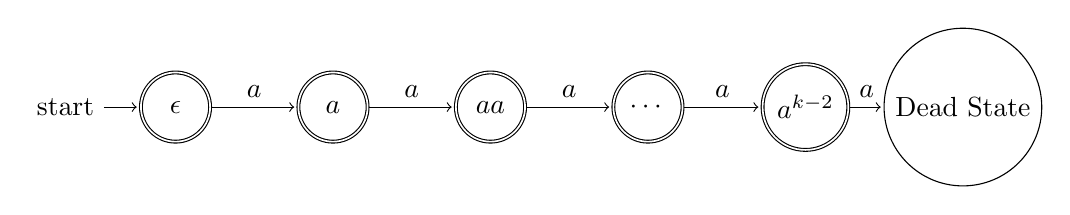
\begin{tikzpicture}[shorten >=1pt,node distance=2cm,on grid,auto] 
                \node[state, initial, accepting] (a_0) {$\epsilon$}; 
                \node[state, accepting] (a) [right=of a_0] {$a$}; 
                \node[state, accepting] (aa) [right=of a] {$aa$}; 
                \node[state, accepting] (a_dots) [right=of aa] {$\cdots$}; 
                \node[state, accepting] (a_{k-2}) [right=of a_dots] {$a^{k-2}$}; 
                \node[state] (dead) [right=of a_{k-2}] {Dead State}; 
                \path[->] 
                    (a_0)
                        edge node {$a$} (a)
                    (a)
                        edge node {$a$} (aa)
                    (aa)
                        edge node {$a$} (a_dots)
                    (a_dots)
                        edge node {$a$} (a_{k-2})
                    (a_{k-2})
                        edge node {$a$} (dead);
            \end{tikzpicture}
            \caption{DFA, \(A\)}
            \label{fig:automataA}
        \end{figure}

        As we can see, there will be one starting state, \(k-2\) additional
        states, and then one dead state. Therefore there are \(1 + (k-2) + 1 = k\) states.
    \end{proof}

    \begin{proof}
        \textbf{Part 2}
        \\
        
        We will prove by contradiction that \(L_k\) cannot be recognized by any DFA with
        \(k-1\) states.
        \\

        Assume that there is a DFA \(A\) with \(k-1\) states that accepts \(L_k\).
        \\
        
        Let \(w = a^{k-1}\) and therefore \(\left|w\right| = k - 1\). According to the definition, \(w \in L_k\). Let
        the run of \(A\) over \(w\) be \(\rho\). Thus:
        \[
            \begin{split}
                \left|\rho\right| &= \left|w\right| + 1
                \\
                &= k - 1 + 1
                \\
                &= k
            \end{split}
        \]

        Thus according to the pigeonhole principle, the number of states
        reached is equal to \(k\) yet the number of states in \(A\) is only
        \(k - 1\). That means that there exists one state in \(A\) that is visited
        twice. Let's let that state be \(q\).
        \\

        Therefore there exists a \(w'\) such that \(w' \in L_k\) and the run of
        \(A\) over \(w'\) is \(\rho' = q_0 \dots q \dots q \dots q_k\). This is true
        because if a state is visited more than once, there is a loop in \(A\)
        and \(q\) can be visited more than once
        \\

        This is a contradiction because
        \[
            \begin{split}
                \left|w'\right| &\geq \left|w\right| + 1
                \\
                &= (k - 1) + 1
                \\
                &= k
            \end{split}
        \]
        yet the largest string in \(L_k\) has length \(k - 1\) according to the
        definition of \(L_k\). Therefore we have shown that \(L_k\) cannot be
        recognized by any DFA with \(k-1\) states.

    \end{proof}
\end{homeworkProblem}

\pagebreak

\begin{homeworkProblem}
    Let \(L_n\) be the language that "the n-th letter of w from the end is 1"
    for \(n \geq 1\).

    \begin{proof}
        \textbf{Part 1}
        \\

        \(L_n\) can be recognized by a NFA with \(n + 1\) states. To show this,
        we will construct a NFA as such:

        \begin{figure}[here]
            \centering
            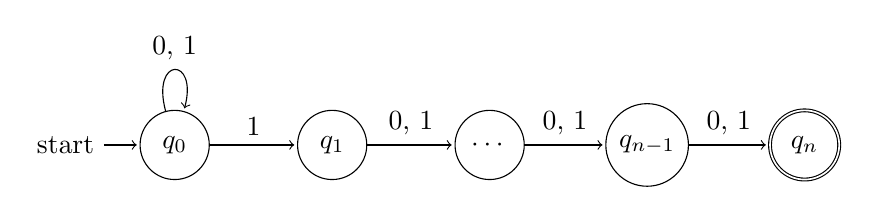
\begin{tikzpicture}[shorten >=1pt,node distance=2cm,on grid,auto] 
                \node[state, initial] (q_0) {$q_0$}; 
                \node[state] (q_1) [right=of q_0] {$q_1$}; 
                \node[state] (q_dots) [right=of q_1] {$\cdots$}; 
                \node[state] (q_{n-1}) [right=of q_dots] {$q_{n-1}$}; 
                \node[state, accepting] (q_n) [right=of q_{n-1}] {$q_n$}; 
                \path[->] 
                    (q_0)
                        edge [loop above] node {0, 1} (q_1)
                        edge node {1} (q_1)
                    (q_1)
                        edge node {0, 1} (q_dots)
                    (q_dots)
                        edge node {0, 1} (q_{n-1})
                    (q_{n-1})
                        edge node {0, 1} (q_n);
            \end{tikzpicture}
            \caption{NFA, \(A\)}
            \label{fig:automataNFA}
        \end{figure}

        As we can see, there will be one state that accepts both 0s and 1s,
        since it is an NFA we can nondeterministically skip to when the nth
        spot of a word is 1 and accept it. We can also see that to do so it
        requires one initial state, and then \(n\) states to transition through
        once there is a 1 in the nth spot. Therefore the number of states = \(n + 1\).

    \end{proof}

    \begin{proof}
        \textbf{Part 2}
        \\
        
        We will prove that any DFA that recognizes \(L_n\) needs at least \(2^n\).

        Assume there is a DFA, \(A\) with less than \(2^n\) states that accepts \(L_n\).
        Let \(A = (Q, \Sigma, \delta, q_0, F)\).
        \\

        The number of strings when we have \(n\) is equal to \(2^n\) since our
        alphabet is binary.
        \\

        Since there are \(2^n - 1\) states yet \(2^n\) strings, there must be
        two strings (according to the pigeonhole principle) such that they end
        on the same state. Or more formally \(\delta(q_0, w) = \delta(q_0, w')\).
        \\

        Since \(w, w'\) are the same length, there must be a point in each
        string where they differ from each other. Because of this, \(A\) cannot
        accept both \(w, w'\).
        \\

        Similar to problem 4, continuing this gives us a contradiction because either
        \(A\) accepts both words or it rejects both.

    \end{proof}
\end{homeworkProblem}

\end{document}
